\chapter{Résolution du système linéaire}

\paragraph{}
On s'intéresse dans ce chapitre à la résolution numérique d'un système linéaire $Ax = b$, de taille $N$.
On cherche donc $x\in\mathbb{K}^N$ avec le second membre $b\in\mathbb{K}^N$ et la matrice $A\in\matrixsymb{N}{K}$ connus.
Dans le cadre de l'énergétique et de la multi-physique, les équations sont réelles mais pour plus de généralité dans la suite on prend le corps $\mathbb{K} = \mathbb{R}\textrm{ ou }\mathbb{C}$.


\section{Contexte de résolution}

	\subsection{Système linéaire creux}

	\paragraph{}
	Comme cela a été mentionné, la taille des matrices rencontrées dans un problème typique de la simulation numérique de la dynamique des fluides est très grande.
	Les matrices ont également une autre propriété : la creusité.
	Puisque les matrices des systèmes linéaires à résoudre sont liées à une matrice jacobienne (voir équation (\ref{eq:linear})), un coefficient de la matrice symbolise une interaction entre deux points du maillage.
	On comprend alors que si le graphe de ces interactions dépend du schéma de discrétisation et d'intégration spatiale, deux points éloignés dans le maillage ne seront normalement pas reliés.
	Ainsi, les matrices présentent cette caractéristique notable qu'est la creusité et que l'on peut observer sur la figure \ref{fig:sparse}.
	On y voit en effet que la majorité des coefficients du système linéaire sont 0.
	En pratique, les matrices rencontrées sont tellement grandes qu'il n'est pas possible de les stocker et de les utiliser sous leur forme dense.
	La propriété de creusité permettra d'utiliser des représentation astucieuses pour stocker les matrices en mémoire, telle que le format CSR (Compressed Sparse Row) \cite{Saad2003}.
	Ces formats permettent à la fois d'économiser de l'espace en mémoire lors du stockage de la matrice, mais également de réaliser des opérations telles que le produit matrice vecteur plus efficacement qu'avec une matrice dense de même taille.

	\begin{figure}
		\centering
		\begin{subfigure}[t]{0.3\textwidth}
			\centering
			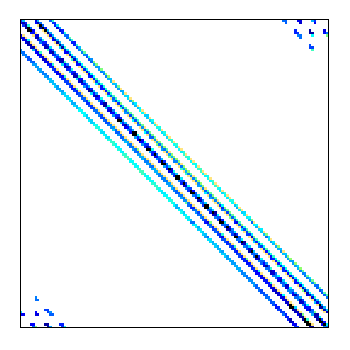
\includegraphics[width=\textwidth]{images/GT01R.png}
			\caption{GT01R : écoulement 2D non visqueux à travers un étage d'aubes de turbomachine}
			\label{fig:sparse.GT01R}
		\end{subfigure}
		\hfill
		\begin{subfigure}[t]{0.3\textwidth}
			\centering
			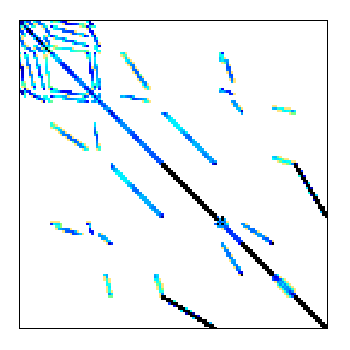
\includegraphics[width=\textwidth]{images/HV15R.png}
			\caption{HV15R : écoulement RANS 3D dans la soufflante d'un moteur}
			\label{fig:sparse.HV15R}
		\end{subfigure}
		\hfill
		\begin{subfigure}[t]{0.3\textwidth}
			\centering
			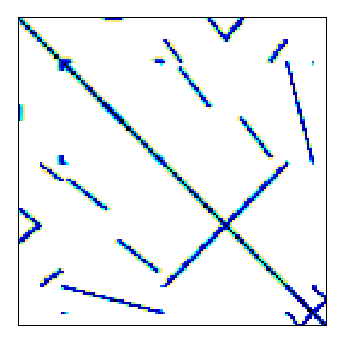
\includegraphics[width=\textwidth]{images/RM07R.png}
			\caption{RM07R : écoulement 3D visqueux dans le compresseur d'un turbopropulseur}
			\label{fig:sparse.RM07R}
		\end{subfigure}
		\caption{Représentation de matrices issues de problèmes de CFD \cite{PacullAubertBuisson2011}, utilisant une méthode spatiale Volumes Finis, les points de couleurs correspondant aux valeurs non nulles}
		\label{fig:sparse}
	\end{figure}


	\subsection{Type de méthode}

		\paragraph{}
		Il existe un grand nombre de méthodes pour inverser un problème linéaire.
		Cependant, en simulation numérique de la dynamique des fluides, la taille des maillage est souvent très importante (\PS{PAR EXEMPLE ?}), ce qui engendre des systèmes de très grande taille.
		Certaines méthodes de résolution ne sont alors plus compatibles, comme en particulier les méthodes directes.
		Cette famille de méthodes, dont fait partie par exemple la méthode du pivot de Gauss, calcule exactement la solution du système linéaire, mais nécessite un temps de calcul très important et un espace mémoire déraisonnable pour les tailles de nos problèmes.
		À l'inverse, les méthodes itératives produisent une suite de vecteurs qui convergent vers la solution du système linéaire.
		L'erreur sur la résolution du système décroît à mesure que l'algorithme itère et cela permet d'atteindre la précision souhaitée, non nulle mais suffisamment petite, pour un temps de calcul et une consommation mémoire maîtrisé.
		C'est l'idée que l'on retrouve sur la figure \ref{fig:direct-iterative} : la méthode directe ne fait aucun progrès avant $O\left(N^3\right)$ opérations, alors que la norme de l'erreur décroît avec le numéro d'itération pour la méthode itérative.

		\begin{figure}
			\centering
			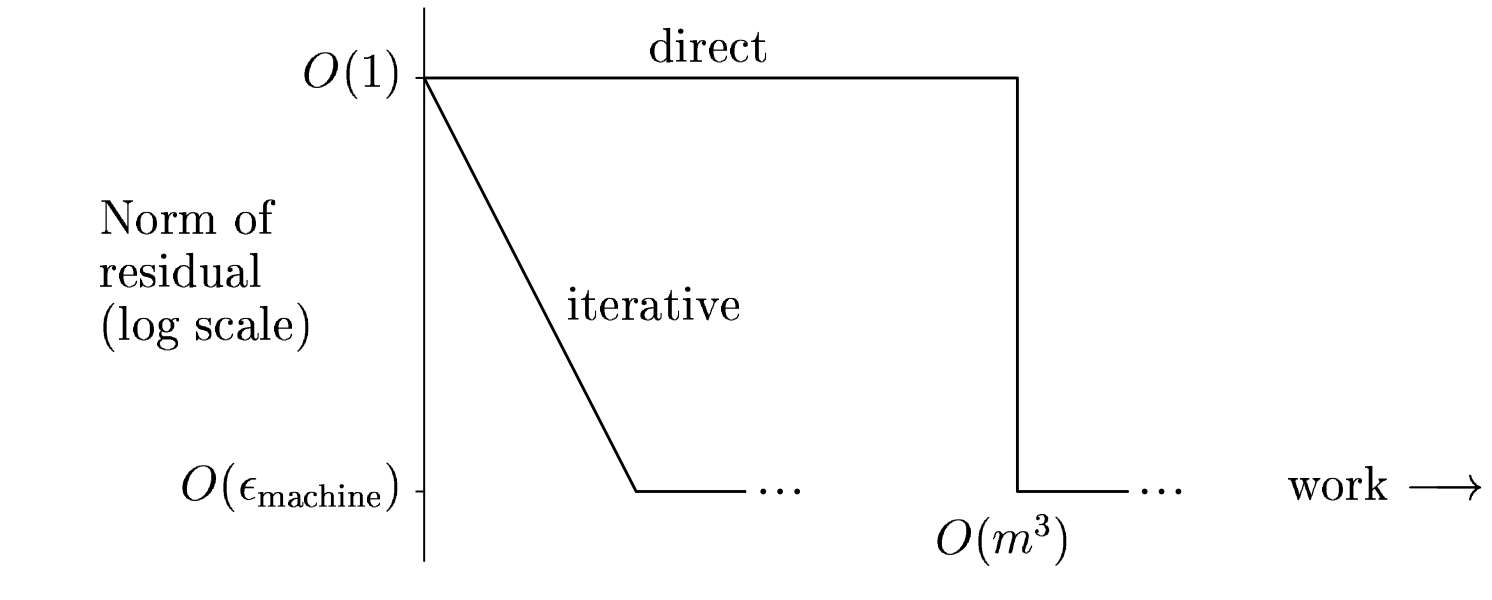
\includegraphics[width=.7\textwidth]{images/direct-iterative.png}
			\caption{Convergence des méthodes directes et itératives, issu de \cite{TrefethenBau1997}}
			\label{fig:direct-iterative}
		\end{figure}

		\paragraph{}
		Les méthodes itératives sont donc les plus adaptées pour inverser des systèmes linéaires creux de grande taille.
		Cependant, il peut arriver qu'on utilise une méthode directe : on peut envisager par exemple la résolution d'un système linéaire avec une succession d'étages d'un algorithme multigrille, pour arriver à un système grossier de petite taille (ou du moins de taille raisonnable), qu'on résoudrait avec une méthode directe comme la décomposition LU.
		Ces méthodes sont bien connues \cite{TrefethenBau1997}, et ne seront pas détaillées ici.


	\subsection{Méthodes itératives}

		\paragraph{}
		Les méthodes itératives sont encore aujourd'hui très étudiées dans la communauté des mathématiques appliquées \cite{OlshanskiiTyrtyshnikov2014, Saad2003, TrefethenBau1997}.
		Une première classe de méthode intervient : les méthodes itératives classiques.
		Si ces méthodes sont plutôt anciennes et plutôt écartées pour leurs mauvaises performances, elles peuvent s'utiliser en se combinant avec des méthodes plus efficaces, et c'est pour cela qu'il est important de comprendre leur fonctionnement.
		Ce sont des méthodes de relaxation, parmi lesquelles on compte les méthode de Jacobi, Gauss-Seidel ou encore SOR (Successive Over Relaxation).
		Leur fonctionnement réside dans une décomposition $A = M - N$ avec $M$ une matrice relativement facile à inverser, où le choix de la décomposition est propre à la méthode.
		Pour la méthode de Jacobi on prendra pour $M$ la diagonale de $A$.
		Il suffit ensuite, à partir d'un itéré initial $x_0$ d'appliquer la formule de récurrence $x_{k+1} = M^{-1}\left(Nx_k + b\right)$.
		Cependant, comme dit précédemment, ces méthodes n'offrent pas une convergence satisfaisante pour la communauté de CFD.
		Ainsi, il faut se tourner vers un autre type de méthodes itératives pour résoudre le système linéaire.


\section{Méthodes de Krylov}

	\subsection{Principe des méthodes}

		\paragraph{}
		Les méthodes de Krylov s'imposent comme étant la norme dans le domaine de la dynamique des fluides numérique.
		Le principe d'une méthode de Krylov est de projeter le système linéaire sur un espace restreint appelé espace de Krylov, et d'y résoudre le système maintenant qu'il est plus petit.
		L'astuce va être dans le fait que ces espaces de Krylov sont emboîtés, et qu'a chaque nouvelle itération on utilise l'information accumulée lors des précédentes.

		\paragraph{}
		Dans ce qui suit, on notera à l'itération $n$ le résidu $r_n = b - Ax_n$, où $x_n$ est l'itéré produit par l'algorithme.
		Dans la pratique, on se restreint à un nombre d'itérations $n\ll N$ pour des raisons évoquées précédemment, mais la suite reste vraie pour $n\le N$.
		On supposera également que l'équation (\ref{eq:linear}) admet une solution.
		Enfin, on notera que résoudre $Ax = b$ avec un itéré initial $x_0$ est équivalent ici à résoudre $A\tilde{x} = b - Ax_0$ avec un itéré initial nul, puis à prendre $x_0 + \tilde{x}$ comme vecteur solution.

		\paragraph{}
		Pour résoudre $Ax = b$ en partant d'un itéré initial $x_0$ et donc d'un résidu $r_0 = b - Ax_0$, on définit l'espace de Krylov à l'itération $n$:
		\begin{equation}\label{eqn:krylov}
			\krylov[A, r_0]{n} = \operatorname{Vect}\left(r_0, Ar_0, \dots, A^{n-1}r_0\right)\ .
		\end{equation}
		On constate alors que par définition $\krylov{1}\subset\krylov{2}\subset\dots\subset\krylov{n-1}\subset\krylov{n}$.
		On cherche ensuite l'itéré sur $\krylov{n}$ qui garantit une condition de Petrov-Galerkin \cite{SimonciniSzyld2007} :
		\begin{equation}\label{eqn:x_n}
			x_n \in x_0 + \krylov[A, r_0]{n}\quad\textrm{tel que}\quad x_n \perp \mathcal{L}_n
		\end{equation}
		où $\mathcal{L}_n$ est un sous-espace vectoriel de dimension $n$.
		Pour $\mathcal{L}_n = \krylov{n}$ on parle de condition de Galerkin, et pour $\mathcal{L}_n = A\krylov{n}$ de minimisation du résidu.
		On voit donc que si $A$ est inversible, $\mathcal{L}_N = \mathbb{K}^N$ et alors l'algorithme termine en au plus $N$ itérations.
		Cette remarque n'a pas grand intérêt en pratique puisqu'on arrêtera l'algorithme bien avant.

		\paragraph{}
		Pour construire les différents espaces de Krylov, on utilise l'itération d'Arnoldi \cite{TrefethenBau1997}.
		La matrice $A$ est semblable à une matrice de Hessenberg $H$ :
		\begin{equation}\label{eq:hessenberg}
			A = VH\adj{V}\Leftrightarrow AV = VH\quad\textrm{avec}\quad H=
			\begin{pmatrix}
				h_{1,1}&h_{1,2}&h_{1,3}&\cdots &h_{1,N}\\
				h_{2,1}&h_{2,2}&h_{2,3}&\cdots &h_{2,N}\\
				0      &h_{3,2}&h_{3,3}&\cdots &h_{3,N}\\
				\vdots &\ddots &\ddots &\ddots &\vdots \\
				0      &\cdots &0      &h_{N,N-1}&h_{N,N}
			\end{pmatrix}\ .
		\end{equation}
		Dans (\ref{eq:hessenberg}), $V$ est une matrice orthonormale de taille $N$.
		On notera $v_i$ sa $i^{\textrm{ème}}$ colonne.
		On notera également $V_n\in\matrixsymb{N, n}{K}$ la matrice constituée des $n$ premières colonnes de $V$.
		On notera enfin $\widetilde{H}_n\in\matrixsymb{n+1, n}{K}$ le bloc supérieur gauche de $H$, qui est également de Hessenberg.

		\paragraph{}
		En considérant les $n \le N$ premières colonnes de (\ref{eq:hessenberg}), de par la structure de Hessenberg de $H$, on obtient la relation d'Arnoldi :
		\begin{equation}\label{eq:arnoldi}
			AV_n = V_{n+1}\widetilde{H}_n
		\end{equation}
		et en considérant la dernière colonne de l'équation (\ref{eq:arnoldi}) :
		\begin{equation}\label{eq:arnoldi_n+1}
			Av_n = h_{1,n}v_1 + \dots + h_{n,n}v_n + h_{n+1,n}v_{n+1}\ .
		\end{equation}

		\paragraph{}
		On peut maintenant décrire l'algorithme :
		Puisque $\krylov{1} = \operatorname{Vect}\left(r_0\right)$, on pose $v_1 = \frac{r_0}{\norm{r_0}}$.
		On itère ensuite sur $n$ : en connaissant $V_n$, la relation (\ref{eq:arnoldi_n+1}) permet de trouver le nouveau vecteur de base et la $n$\textsuperscript{ième} colonne de $H$, c'est à dire de trouver $V_{n+1}$ et $\widetilde{H}_n$.
		Les espaces vectoriels $\operatorname{Im}\left(V_n\right)$ sont alors par construction les espaces de Krylov $\krylov{n}$.

		\paragraph{}
		On remarque que la matrice $A$ n'intervient dans la relation (\ref{eq:arnoldi_n+1}) qu'à travers le produit $Av_n$.
		Il n'est donc pas nécessaire de former explicitement la matrice du système linéaire, mais seulement de pouvoir calculer son action sur un vecteur.
		Cette propriété des méthodes de Krylov sera utilisée par la suite.

		\paragraph{}
		Il existe donc beaucoup de méthodes de Krylov pour résoudre un système linéaire, la principale distinction entre elle se faisant par le choix du sous-espace $\mathcal{L}_n$.
		La condition de minimisation du résidu donne la méthode GMRES, qui est l'une des plus utilisée par les communautés de CFD et de mathématiques appliquées.
		Elle permet, après des itérations un peu plus coûteuses que ses consœurs telles que la méthode Bi-CG \cite{TrefethenBau1997}, de minimiser le résidu obtenu et donc de garantir la décroissance de l'erreur.
		De plus, la méthode GMRES est beaucoup étudiée et de nombreuses variantes et améliorations ont été développées au fil des années.
		Pour ces raisons, et parce que son implémentation est relativement simple, c'est sur cette méthode que j'ai décidé de m'orienter.


	\subsection{GMRES}

		\paragraph{}
		La méthode GMRES consiste donc, à chaque itération $n$, à :
		\begin{itemize}
			\item calculer le nouvel espace de Krylov $\krylov{n+1}$ à partir de $\krylov{n}$, donc d'après (\ref{eq:arnoldi_n+1}) de calculer le produit $Av_n$, puis de l'orthonormaliser sur les colonnes de $V_n$ pour obtenir $\widetilde{H}_n$ et $V_{n+1}$
			\item trouver $x_n \in x_0 + \krylov{n}$ qui minimise la norme de $r_n = b - Ax_n$.
		\end{itemize}
		Puisque $x_n \in x_0 + \krylov{n}$, $x_n = x_0 + V_n y_n$ pour un certain $y_n\in\mathbb{K}^n$.
		On dispose de la relation d'Arnoldi (\ref{eq:arnoldi}), donc :
		\begin{align*}
			\norm{r_n} &= \norm{b - Ax_n} \\
			&= \norm{r_0 - AV_ny_n} \\
			&= \norm{r_0 - V_{n+1}\widetilde{H}_ny_n} \\
			&= \norm{\norm{r_0} e_1 - \widetilde{H}_ny_n}\qquad\textrm{avec $e_1$ le premier vecteur de la base canonique de $\mathbb{K}^{n+1}$.}
		\end{align*}

		\paragraph{}
		La condition de minimisation du résidu est remplie en résolvant un problème de minimisation de taille $n$.
		En pratique ce problème est résolu par décomposition QR de la matrice de Hessenberg.
		Pour ce faire, on suppose qu'on dispose d'une décomposition $\Omega_n\widetilde{H}_n = \begin{pmatrix}R_n \\ 0\end{pmatrix}$ avec $\Omega_n\in\orthogroup{n+1}{K}$ une matrice unitaire et $R_n\in\matrixsymb{n}{K}$ une matrice diagonale.
		La décomposition QR de $\widetilde{H}_n$ à en effet cette forme de par sa structure de Hessenberg.
		C'est le cas à l'itération 1 avec $\Omega_1 = \operatorname{Id}$ et $R_1 = 1$.
		On note ensuite :
		\[\begin{pmatrix}\Omega_n & 0 \\ 0 & 1\end{pmatrix}\widetilde{H}_{n+1} = \begin{pmatrix}R_n & r_{n+1} \\ 0 & \rho \\ 0 & \sigma\end{pmatrix} \quad\textrm{avec}\quad \begin{pmatrix}r_{n+1} \\ \rho\end{pmatrix} = \Omega_n\begin{pmatrix}h_{n,n+1} \\ \vdots \\ h_{n+1,n+1}\end{pmatrix} \quad\textrm{et}\quad \sigma = h_{n+2,n+1}\ .\]
		On pose ensuite la rotation de Givens :
		\[G_n = \left\{\begin{aligned}
			&\quad\operatorname{Id}_{n+2} &\textrm{si }\rho = \sigma = 0\\ \\
			\begin{pmatrix}\operatorname{Id}_n & 0 & 0 \\ 0 & c & s \\ 0 & -s & c\end{pmatrix}& \quad\textrm{avec}\quad c = \frac{\rho}{\sqrt{\rho^2 + \sigma^2}}, s = \frac{\sigma}{\sqrt{\rho^2 + \sigma^2}} &\quad\textrm{sinon.}
		\end{aligned}\right.\]
		On remarque enfin que :
		\[G_n\begin{pmatrix}\Omega_n & 0 \\ 0 & 1\end{pmatrix}\widetilde{H}_{n+1} = \begin{pmatrix}R_n & r_{n+1} \\ 0 & \sqrt{\rho^2 + \sigma^2} \\ 0 & 0\end{pmatrix}\]
		ce qui donne la nouvelle décomposition QR : $\Omega_{n+1}\widetilde{H}_{n+1} = \begin{pmatrix}R_{n+1} \\ 0\end{pmatrix}$.


		\paragraph{}
		Finalement, la décomposition QR de la matrice de Hessenberg se construit à mesure des itérations, de manière peu coûteuse.
		Cette décomposition est cependant très intéressante.
		Lorsqu'on cherche à minimiser le résidu, on à montré précédemment qu'on minimise :
		\begin{align*}
			\norm{r_n} &= \norm{\norm{r_0} e_1 - \widetilde{H}_ny_n} \\
			&= \norm{\norm{r_0} \Omega_ne_1 - \begin{pmatrix}R_ny_n \\ 0\end{pmatrix}}\ .
		\end{align*}
		La solution de ce problème de minimisation est connu.
		En notant $\Omega_ne_1 = \begin{pmatrix}\omega_1 \\ \omega_{1n}\end{pmatrix}$ la première colonne de $\Omega_n$, on a :
		\[y_n = \norm{r_0}R_n^{-1}\omega_1\quad\textrm{et}\quad\norm{r_n} = \norm{r_0}\left|\omega_{1n}\right|\ .\]
		L'intérêt de mettre à jour la décomposition de la matrice de Hessenberg est alors double :
		\begin{itemize}
			\item l'inversion du système réduit est explicite, par inversion d'une matrice triangulaire ce qui est aisé
			\item la norme du résidu peut être calculée à chaque itération sans inverser le système, ce qui permet un meilleur contrôle des itérations.
		\end{itemize}

		\paragraph{}
		Mon choix s'est porté sur la méthode GMRES pour plusieurs raisons.
		Tout d'abord, c'est une méthode de Krylov, et le choix de ce type de méthode a déjà été argumenté précédemment.
		Ensuite, cette méthode permet un contrôle du résidu, car la norme de celui ci décroît entre chaque itération.
		Ce n'est pas le cas pour toutes les méthodes de Krylov comme par exemple pour la méthode Bi-CG.
		GMRES est un algorithme relativement simple qui ne nécessite pas (ou peu) de réglages, que ce soit de la part du développeur ou bien de l'utilisateur.
		Cette méthode de résolution du système linéaire est encore aujourd'hui bien présente au sein de la communauté de mathématiques appliquées \cite{Vasseur2016}, de CFD \cite{FrancoCamierAndrejEtAl2020} et est utilisée dans bien d'autres domaines, comme par exemple l'électromagnétisme \cite{ErnstGander2012} ou la mécanique du solide \cite{Mercier2015}.


	\subsection{Convergence des méthodes}

		\paragraph{}
		La convergence des méthodes de Krylov, et plus généralement des méthodes itératives, dépend du système linéaire.
		En effet, si une méthode itérative fait converger la norme de l'erreur ou celle du résidu vers 0, la vitesse de convergence dépend à la fois de la méthode et de la matrice à inverser.

		\paragraph{}
		On se rend compte en parcourant la litérature a convergence des méthode itératives est très fortement liée au conditionnement de l'opérateur $A$.
		Le conditionnement d'une matrice inversible $A$ est :
		\[\kappa\left(A\right) = \norm{A}\norm{A^{-1}}\]
		et dépend donc de la norme choisie.
		Une matrice dite bien conditionnée, du point de vue des algorithmes itératifs, a un conditionnement $\kappa = O\left(1\right)$.
		Au contraire, pour une matrice mal conditionnée, $\kappa\gg1$.

		\paragraph{}
		Pour la norme $\norm[2]{\cdot}$ on a, pour une matrice $A$ :
		\begin{equation}\label{eq:conditionnement}
			\kappa\left(A\right) = \frac{\sigma_{\max}}{\sigma_{\min}}
		\end{equation}
		où $\sigma_{\min}$ et $\sigma_{\max}$ sont les valeurs singulières minimales et maximales de $A$.
		Pour rappel, les valeurs singulières de $A$ sont les valeurs propres de $\adj{A}A$.

		\paragraph{}
		On trouve souvent la relation : $\kappa\left(A\right) = \frac{\left|\lambda_{\max}\right|}{\left|\lambda_{\min}\right|}$ avec $\lambda_{\min}$ et $\lambda_{\max}$ les valeurs propres de $A$ de plus petit et de plus grand module.
		Cependant cette relation n'est vraie que pour les matrices normales (qui commutent avec leur matrice adjointe).
		Pour cette raison, il ne sert à rien de se baser uniquement sur le spectre de l'opérateur pour étudier la convergence des méthodes.

		\paragraph{}
		Dans \cite{GreenbaumPtakStrakos1996}, on trouve un résultat surprenant.
		Cet article montre en effet que pour un spectre donné et pour une courbe de convergence décroissante donnée, il est possible de construire une matrice avec ce spectre telle que GMRES suivra la courbe de convergence.
		Autrement dit, on peut exhiber un exemple de matrice mal conditionnée qui converge rapidement, et à l'inverse trouver une matrice bien conditionnée pour laquelle GMRES aura du mal à faire décroitre le résidu.
		Ce phénomène est causé par la non-normalité de l'opérateur \cite{GreenbaumStrakos1994, GreenbaumPtakStrakos1996, Trefethen1999}.
		Puisque les matrices rencontrées dans les problèmes de CFD sont quelconques, ou au moins à priori non-normales, étudier précisément le spectre de l'opérateur ne semble pas être une bonne idée.

		\paragraph{}
		Si une étude précise du spectre de la matrice n'est pas recomandée, une rapide analyse peut toutefois s'avérer utile.
		En effet, mathématiquement parlant, le spectre peut ne donner aucune information, d'après le paragraphe précédent.
		Cependant, les matrices rencontrées en pratiques ne sont pas des contres-exemples d'une preuve mathématique, mais de vraies matrices quelconque.
		En faisant l'hypothèse qu'on ne tombera pas précisément sur un cas particulier, on peut continuer à regarder le spectre de $A$ pour se donner une idée de la convergence de l'algorithme.


\section{Améliorations de l’algorithme}

	\paragraph{}
	Dans la suite on suppose qu'on dispose d'une méthode de résolution du problème linéaire (\ref{eq:linear}).
	Conformément à ce qui a été argumenté dans les parties précédentes, on prendra donc une méthode de Krylov : la méthode GMRES.
	Nous pouvons déjà appliquer cette méthode pour obtenir une solution au système linéaire, cependant il est possible de faire mieux.
	En effet, la méthode GMRES peut être améliorée, affinée, pour obtenir plus efficacement la solution.
	De telles améliorations sont présentées dans ce qui suit.
	Il sera précisé si cette amélioration concerne typiquement la méthode GMRES, ou si elle s'applique généralement à toute méthode de résolution d'un système linéaire.
